\documentclass[11pt]{article}

\newcommand{\yourname}{Kevin Zhang}

\def\comments{0}

%format and packages

%\usepackage{algorithm, algorithmic}
\usepackage{forest}
\usepackage{tikz}
\usepackage{algpseudocode}
\usepackage{amsmath, amssymb, amsthm}
\usepackage{tcolorbox}
\usepackage{enumerate}
\usepackage{enumitem}
\usepackage{framed}
\usepackage{verbatim}
\usepackage[margin=1.0in]{geometry}
\usepackage{microtype}
\usepackage{kpfonts}
\usepackage{url}
\usepackage{palatino}
	\DeclareMathAlphabet{\mathtt}{OT1}{cmtt}{m}{n}
	\SetMathAlphabet{\mathtt}{bold}{OT1}{cmtt}{bx}{n}
	\DeclareMathAlphabet{\mathsf}{OT1}{cmss}{m}{n}
	\SetMathAlphabet{\mathsf}{bold}{OT1}{cmss}{bx}{n}
	\renewcommand*\ttdefault{cmtt}
	\renewcommand*\sfdefault{cmss}
	\renewcommand{\baselinestretch}{1.06}

\usepackage[boxruled,vlined,nofillcomment]{algorithm2e}
	\SetKwProg{Fn}{Function}{\string:}{}
	\SetKwFor{While}{While}{}{}
	\SetKwFor{For}{For}{}{}
	\SetKwIF{If}{ElseIf}{Else}{If}{:}{ElseIf}{Else}{:}
	\SetKw{Return}{Return}
	

%enclosure macros
\newcommand{\paren}[1]{\ensuremath{\left( {#1} \right)}}
\newcommand{\bracket}[1]{\ensuremath{\left\{ {#1} \right\}}}
\renewcommand{\sb}[1]{\ensuremath{\left[ {#1} \right\]}}
\newcommand{\ab}[1]{\ensuremath{\left\langle {#1} \right\rangle}}

%probability macros
\newcommand{\ex}[2]{{\ifx&#1& \mathbb{E} \else \underset{#1}{\mathbb{E}} \fi \left[#2\right]}}
\newcommand{\pr}[2]{{\ifx&#1& \mathbb{P} \else \underset{#1}{\mathbb{P}} \fi \left[#2\right]}}
\newcommand{\var}[2]{{\ifx&#1& \mathrm{Var} \else \underset{#1}{\mathrm{Var}} \fi \left[#2\right]}}

%useful CS macros
\newcommand{\poly}{\mathrm{poly}}
\newcommand{\polylog}{\mathrm{polylog}}
\newcommand{\zo}{\{0,1\}}
\newcommand{\pmo}{\{\pm1\}}
\newcommand{\getsr}{\gets_{\mbox{\tiny R}}}
\newcommand{\card}[1]{\left| #1 \right|}
\newcommand{\set}[1]{\left\{#1\right\}}
\newcommand{\negl}{\mathrm{negl}}
\newcommand{\eps}{\varepsilon}
\DeclareMathOperator*{\argmin}{arg\,min}
\DeclareMathOperator*{\argmax}{arg\,max}
\newcommand{\eqand}{\qquad \textrm{and} \qquad}
\newcommand{\ind}[1]{\mathbb{I}\{#1\}}
\newcommand{\sslash}{\ensuremath{\mathbin{/\mkern-3mu/}}}
\newcommand{\pipe}{\hspace{3pt}|\hspace{3pt}}

%mathbb
\newcommand{\N}{\mathbb{N}}
\newcommand{\R}{\mathbb{R}}
\newcommand{\Z}{\mathbb{Z}}
%mathcal
\newcommand{\cA}{\mathcal{A}}
\newcommand{\cB}{\mathcal{B}}
\newcommand{\cC}{\mathcal{C}}
\newcommand{\cD}{\mathcal{D}}
\newcommand{\cE}{\mathcal{E}}
\newcommand{\cF}{\mathcal{F}}
\newcommand{\cL}{\mathcal{L}}
\newcommand{\cM}{\mathcal{M}}
\newcommand{\cO}{\mathcal{O}}
\newcommand{\cP}{\mathcal{P}}
\newcommand{\cQ}{\mathcal{Q}}
\newcommand{\cR}{\mathcal{R}}
\newcommand{\cS}{\mathcal{S}}
\newcommand{\cU}{\mathcal{U}}
\newcommand{\cV}{\mathcal{V}}
\newcommand{\cW}{\mathcal{W}}
\newcommand{\cX}{\mathcal{X}}
\newcommand{\cY}{\mathcal{Y}}
\newcommand{\cZ}{\mathcal{Z}}

%theorem macros
\newtheorem{thm}{Theorem}
\newtheorem{lem}[thm]{Lemma}
\newtheorem{fact}[thm]{Fact}
\newtheorem{clm}[thm]{Claim}
\newtheorem{rem}[thm]{Remark}
\newtheorem{coro}[thm]{Corollary}
\newtheorem{prop}[thm]{Proposition}
\newtheorem{conj}[thm]{Conjecture}

\theoremstyle{definition}
\newtheorem{defn}[thm]{Definition}
\newtheoremstyle{case}{}{}{}{}{}{:}{ }{}
\theoremstyle{case}
\newtheorem{case}{Case}

\theoremstyle{theorem}
\newtheorem{prob}{Problem}
\newtheorem{sol}{Solution}

\tikzset{every picture/.style={line width=0.75pt}} %set default line width to 0.75pt        

\begin{document}
{\large
\noindent Name: \yourname}
\vspace{15pt}

% Problem 1
\begin{prob}
\end{prob}

\begin{enumerate}[label=(\alph*)]

% Part A
\item We are given two sets $P, N$ with $n$ unit vectors on opposite sides of a hyperplane through the origin. $<a,x> = 0$. Moreover, the distance of each
point from the hyperplane is at least $\varepsilon$. Let $S = \{0,a\} \cup P \cup N \cup P' \cup N'$ with $P',N'$ being their respective points reflected across the origin. 
We want to show it is possible to represent the points in $S$ in lower dimension $O(\log n / \varepsilon^2)$ with distances being preserved up to a $1 \pm (\varepsilon / 10)$.

This is possible with the JL Lemma. The JL Lemma states that for $n$ points in $d$ dimensions, it is possible to represent these points in $m = O(\log n / \varepsilon^2)$ dimensions. 
If we plug into our lemma ($n = 4n$ and $\varepsilon = \varepsilon/10$), we end up with a bound of $m = O(100 \log 4 n / \varepsilon^2)$ with distances being preserved up to $1 \pm (\varepsilon / 10)$.
With Big-O notation, we can simplify $m = O(100 \log 4 n / \varepsilon^2) = O(\log n / \varepsilon^2)$. 

%Part B
\item We want to show that the margin for the above transformation is still preserved up to $\varepsilon / 2$. To do so, we will use
the identity $<a,x> = \frac{||a+x||^2 - ||a-x||^2}{4}$. From this, we have the following:

\begin{align*}
  <\frac{T(a)}{||T(a)||}, T(x)> &= \frac{1}{||T(a)||} <T(a), T(x)> \\ 
  <T(a), T(x)> &= \frac{||T(a)+T(x)||^2 - ||T(a)-T(x)||^2}{4} &\stackrel{?}{\geq} \varepsilon / 2 \\
               &= ||T(a)+T(x)||^2 - ||T(a)-T(x)||^2 &\stackrel{?}{\geq} 2\varepsilon  
\end{align*}

From the JL-Lemma, we have that $T(a) = (1 \pm \frac{\epsilon}{10}) \times a$ and that $T(x) = (1 \pm \frac{\epsilon}{10}) \times x$. Since we
want to find the lower bound, we can push the bounds as far as we can go. This nets us:

\begin{align*}
  (1-\frac{\varepsilon}{10})^2||a+x||^2 - (1 + \frac{\varepsilon}{10})^2||a-x||^2 &\stackrel{?}{\geq} 2\varepsilon \\
  (1-\frac{\varepsilon}{10})^2||a+x||^2 \textbf{$ - (1 + \frac{\varepsilon}{10})||a+x||^2$} - (1 + \frac{\varepsilon}{10})^2||a-x||^2 \textbf{$ + (1 + \frac{\varepsilon}{10})||a+x||^2$} &\stackrel{?}{\geq} 2\varepsilon \\
  \left[ (1 - \frac{\varepsilon}{10})^2 - (1 + \frac{\varepsilon}{10})^2 \right]||a+x||^2 + (1 + \frac{\varepsilon}{10})^2\left[ ||a+x||^2 - ||a-x||^2 \right] &\stackrel{?}{\geq} 2\varepsilon
\end{align*}

We can examine this expression piecewise. First, we know that $a^2 - b^2 = (a + b)(a - b)$. 

\[
  \left[ (1 - \frac{\varepsilon}{10})^2 - (1 + \frac{\varepsilon}{10})^2 \right] ||a+x||^2 = (\frac{-4\varepsilon}{10})||a+x||^2 
\]

Next we know that $||a+x||^2 - ||a-x||^2 = 4\varepsilon$. We know this because of the identity $<a,x> = \frac{||a+x||^2 - ||a-x||^2}{4}$. 

\[
  (1 + \frac{\varepsilon}{10})^2\left[ ||a+x||^2 - ||a-x||^2 \right] = 4\varepsilon (1 + \frac{\varepsilon}{10})^2
\]

If combine these expressions, shuffle terms around, and add back in the $\frac{1}{||T(a)||}$ from earlier, we get the following:

\[
  (1 + \frac{\varepsilon}{10})(4\varepsilon) \stackrel{?}{\geq} 2\varepsilon + \frac{(\frac{4\varepsilon}{10})||a+x||^2}{1 + \frac{\varepsilon}{10}}
\]

Even if we stretch $||a+x||^2$ as far as it can go, which is $4$, the RHS is bounded by $4 \varepsilon$. Meanwhile, the LHS is
$4\varepsilon + (\frac{\varepsilon}{10})(4\varepsilon)$. As such, we are done, and we have proved that the margin is still preserved up to $\varepsilon / 2$.

\end{enumerate}

\newpage

% Problem 2
\begin{prob}
\end{prob}

\begin{enumerate}[label=(\alph*)]

% Part A 
\item We are designing an LSH family as follows: A hash function is to pick a random unit vector $v$ from the unit sphere, and then $h(x)$ is the sign of 
$<v,x>$. If $<v,x> = 0$, then the hash value is $1$. We want to express the probability that two unit vectors $x$ and $y$ shared the same hash value (they collide)
as a function of $r$, the distance between $x$ and $y$. 

We can do this by focusing on the 2-dimensional space spanned by $x$ and $y$. The reasoning for this is because we can project $v$ onto this plane and that 
will the primary decider on the hash value. The first thing we want to define is collision. In this case, two vectors $x$ and $y$ collide when $<v,x>$ and $<v,y>$
share the same sign. And in terms of $v$, the regions of $<v,x>$ are defined below: 

\begin{figure}[h!]
  \centering
  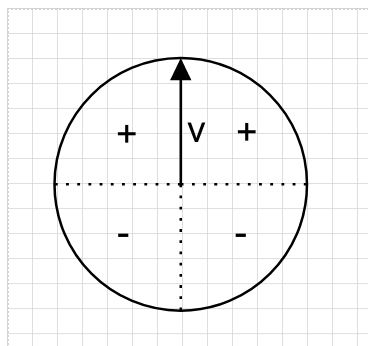
\includegraphics[totalheight=6cm]{images/v-circle.png}
\end{figure}

Thus, in order for $<v,x>$ and $<v,y>$ to share the same sign, $x$ and $y$ must fall into same sign regions. The region that $v$ is allowed to be in 
can be expressed as a function of $\theta$, the angle between vectors $x$ and $y$. This angle of this region is $\pi - \theta$, and can be visualized below:

\begin{figure}[h!]
  \centering
  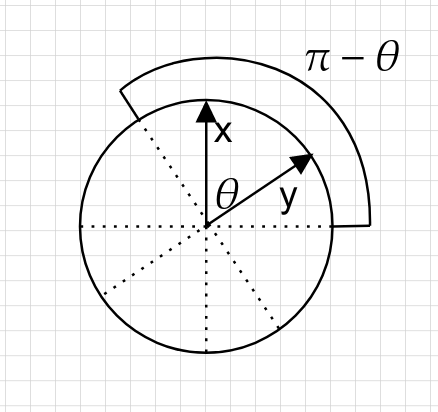
\includegraphics[totalheight=6cm]{images/x-y-circle.png}
\end{figure}

Thus, the probability of collision can be expressed in terms of $\theta$. We double the region size, since we the signs can either be both $+$ or both $-$, and
then divide over the entire circle.

\[
  \text{Pr[collision]} = \frac{2(\pi - \theta)}{2\pi} = 1 - \frac{\theta}{\pi}
\]

To get theta from $r$, we can use the law of cosines:

\begin{align*}
  r^2 &= ||x||^2 + ||y||^2 + 2 ||x|| ||y|| \cos \theta \\
  r^2 &= 1 + 1 + 2 \cos \theta \\
  2 - r^2 &= 2 \cos \theta \\
  \cos \theta &= 1 - \frac{r^2}{2} \\
  \theta &= \arccos{\left( 1 - \frac{r^2}{2} \right) }
\end{align*}

And so, the final probability is:

\[
  \text{Pr[collision]} = 1 - \frac{\arccos{ \left(1 - \frac{r^2}{2} \right) }}{\pi}
\]

% Part B
\item We would like to evaluate the parameter $\rho$ for the approximate near neighbor problem with $c = 2$. If we
let $p_1 = \text{Pr[collision for r]}$ and $p_2 = \text{Pr[collision for 2r]}$ and $\rho = \frac{\log p_1}{\log p_2}$, we
get the following graph:

\begin{figure}[h!]
  \centering
  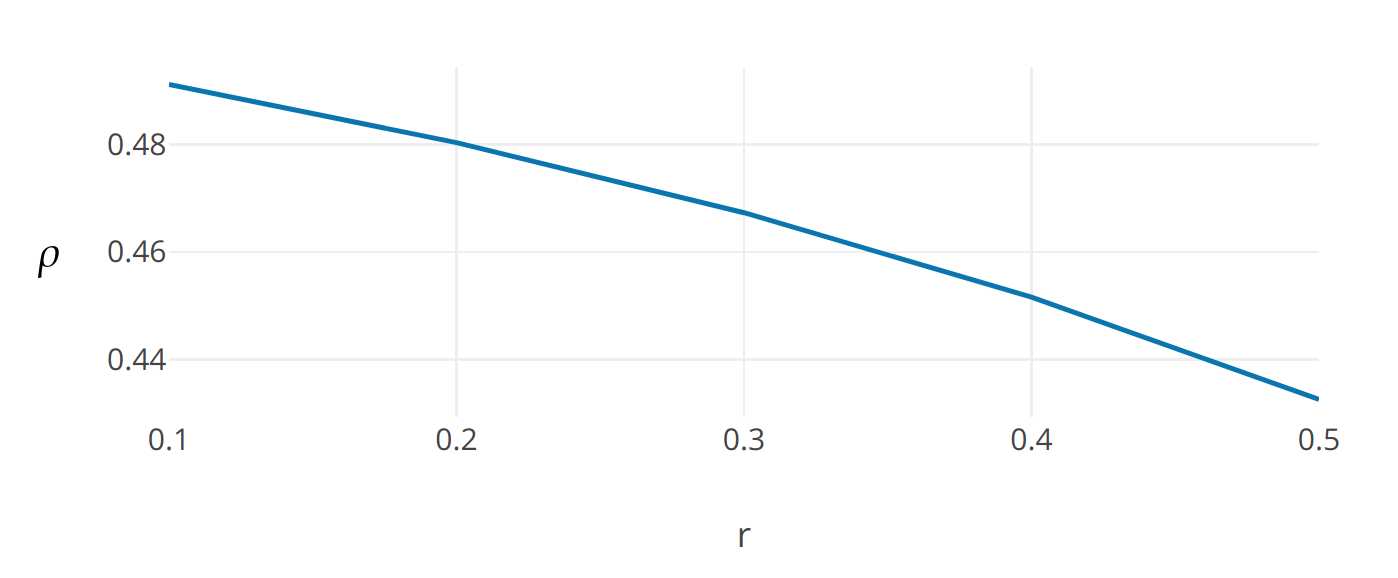
\includegraphics[totalheight=6cm]{images/graph.png}
\end{figure}

\end{enumerate}

\newpage

% Problem 3
\begin{prob}
\end{prob}

Followed the instructions at: https://www.youtube.com/watch?v=H7qMMudo3e8

\begin{verbatim}

from PIL import Image
from matplotlib.image import imread
import matplotlib.pyplot as plt
import numpy as np

# Import image
A = imread('images/sf-gray.jpg')

# SVD computations
U, S, VT = np.linalg.svd(A,full_matrices=False)
S = np.diag(S)

j = 1
for k in (50, 60, 70, 80, 90, 100):
    # appr image
    X = U[:,:k] @ S[0:k,:k] @ VT[:k,:]
    plt.figure(j)
    img = plt.imshow(X)
    img.set_cmap('gray')
    plt.title('k = ' + str(k))
    plt.show()
    j += 1

# Best Approximation
k = 90
B = U[:,:k] @ S[0:k,:k] @ VT[:k,:]
img  = plt.imshow(B)
img.set_cmap('gray')
plt.axis('off')

plt.savefig('images/sf-compressed.jpg')

\end{verbatim}

\newpage

Original Image:

\begin{figure}[h!]
  \centering
  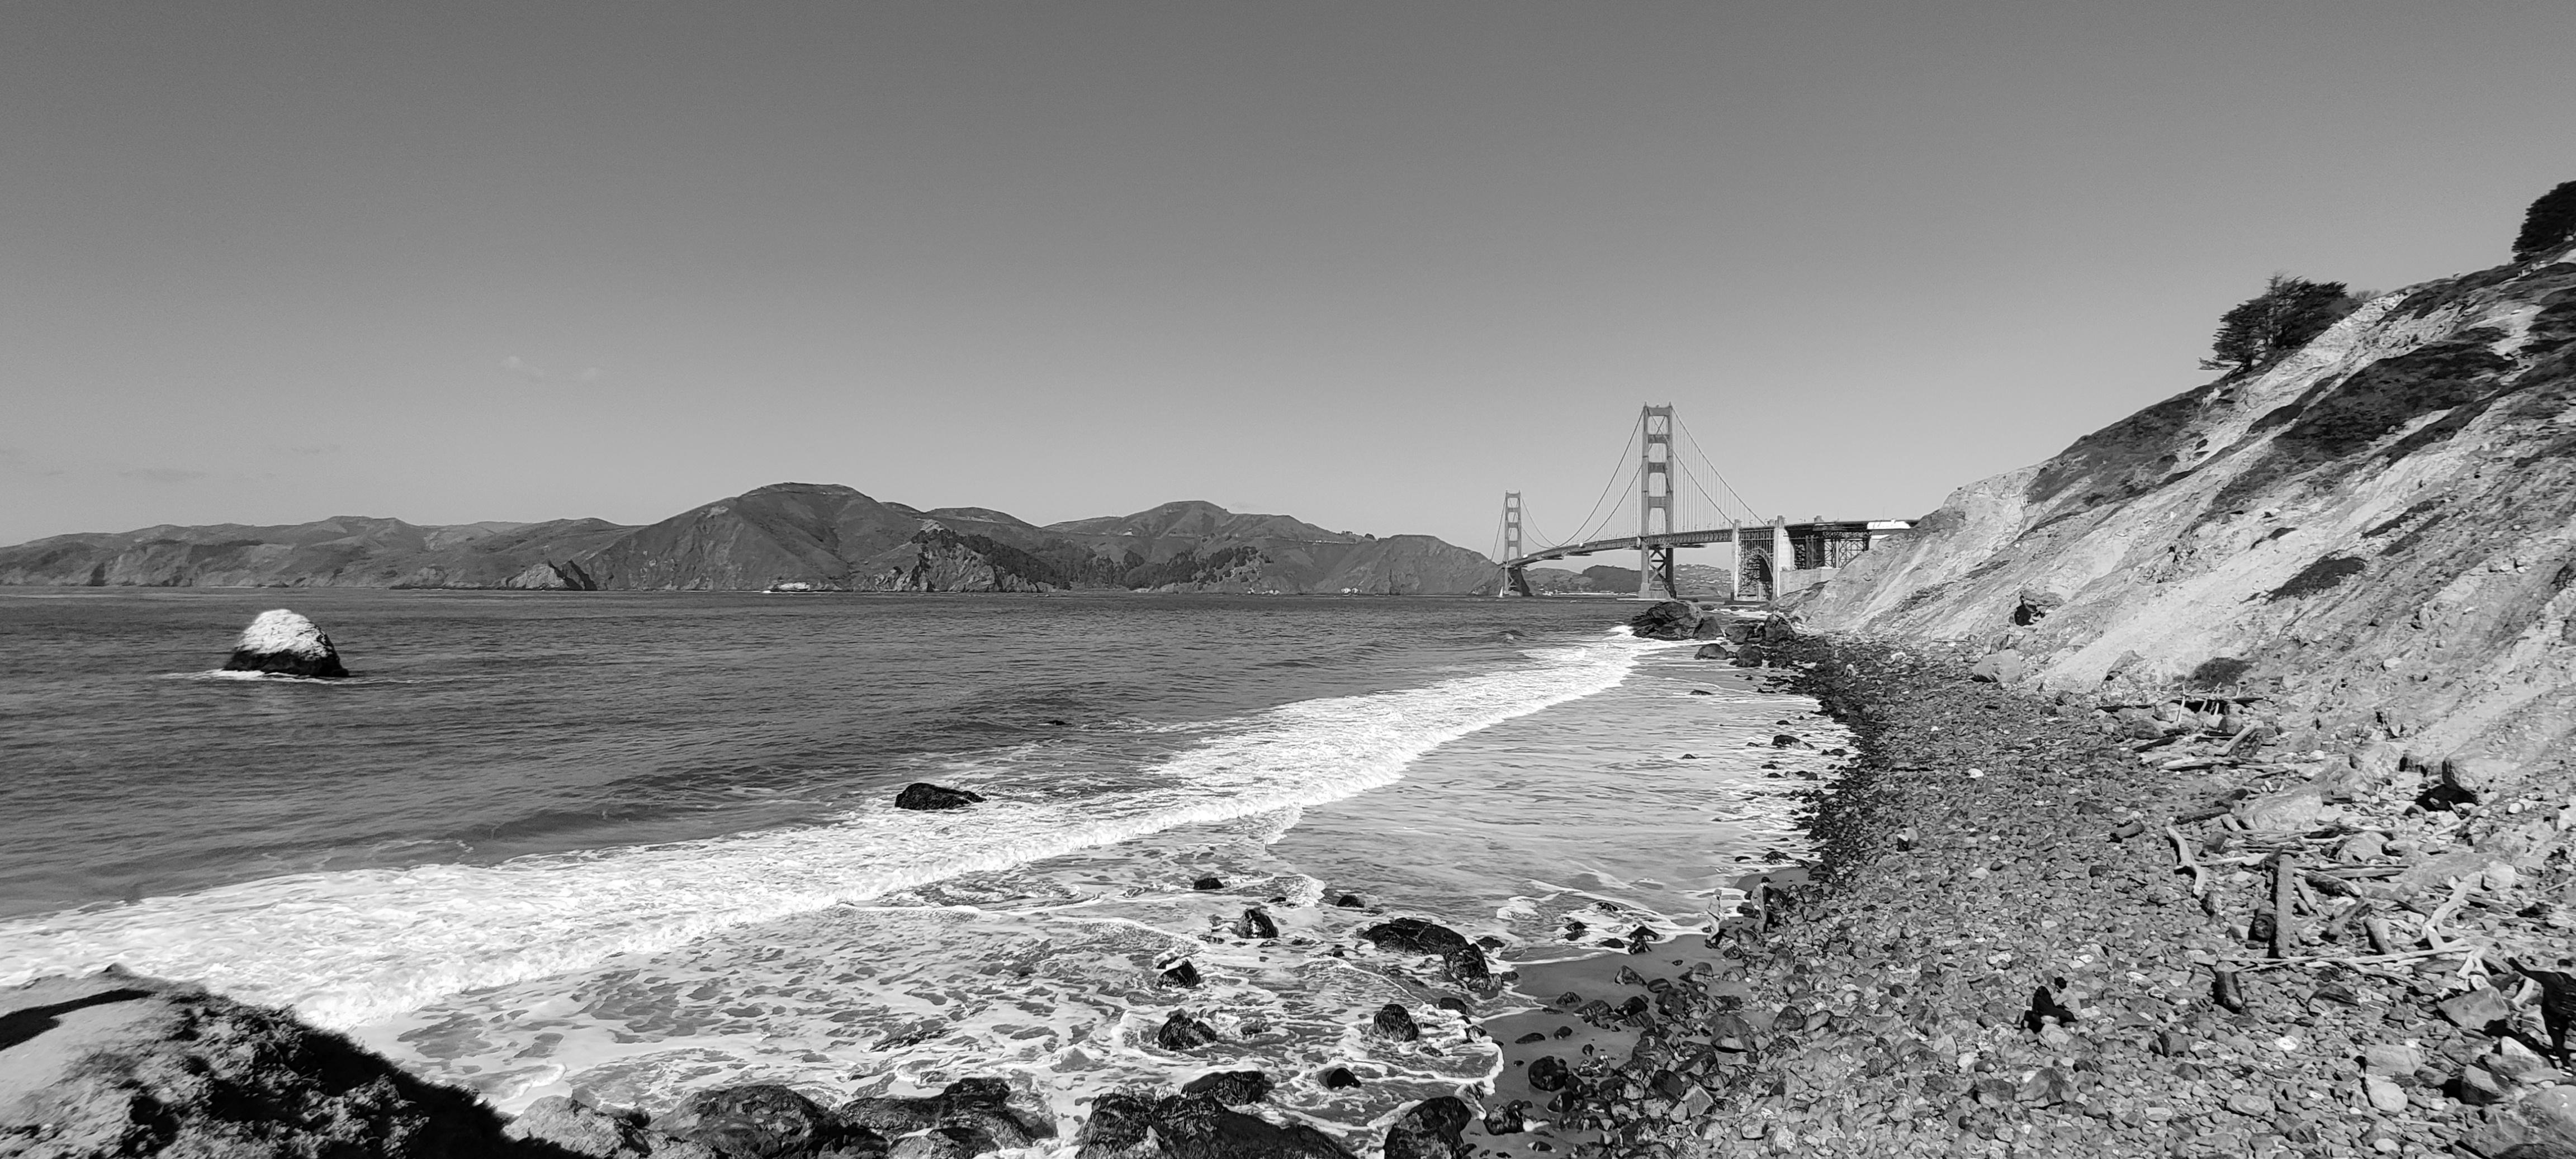
\includegraphics[totalheight=6cm]{images/sf-gray.jpg}
\end{figure}

Compressed Image (at rank 90):

\begin{figure}[h!]
  \centering
  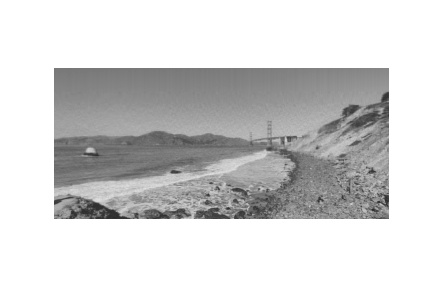
\includegraphics[totalheight=6cm]{images/sf-compressed.jpg}
\end{figure}

\newpage

% Problem 4
\begin{prob}
\end{prob}

\begin{enumerate}[label=(\alph*)]

\item We are given $A = U \Sigma V^T$ with singular values $\sigma_1 \geq \sigma_2 \geq ... \geq \sigma_n$. We would like to find a matrix $B$ 
of at most rank $k$ such that $||A - B||_2 \leq \frac{||A||_F}{\sqrt{k}}$. 

We can define $B$ similarly to $A$, but at rank $k$:

\[
  B = 
  \begin{bmatrix}
    u_1 \\
    u_2 \\
    \vdots \\
    u_n
  \end{bmatrix} 
  \left[
    \begin{array}{ccccccc}
      \sigma_1 & 0        & \hdots & 0        & 0      & \hdots  & 0 \\
      0        & \sigma_2 & \hdots & 0        & 0      & \hdots  & 0 \\
      \vdots   & \vdots   & \ddots & 0        & 0      & \hdots  & 0 \\
      0        & 0        & 0      & \sigma_k & 0      & \hdots  & 0 \\
      0        & 0        & 0      & 0        & 0      & \hdots  & 0 \\
      \vdots   & \vdots   & \vdots & \vdots   & \vdots & \ddots  & 0 \\
      0        & 0        & 0      & 0        & 0      & 0       & 0 
    \end{array}
  \right]
  \begin{bmatrix}
    v_1 \\
    v_2 \\
    \vdots \\
    v_n
  \end{bmatrix}^T
\]

Thus, the result of $||A - B||_2$ can be expressed as follows:

\begin{align*}
  ||A - B||_2 &= \sigma_{k+1} \\
  \sigma_{k+1} &\stackrel{?}{\leq} \frac{||A||_F}{\sqrt{k}} \\
  \sigma_{k+1} &\stackrel{?}{\leq} \frac{\sqrt{\sum_i \sigma_i^2}}{\sqrt{k}} \\
  \sigma_{k+1}^2 &\stackrel{?}{\leq} \frac{\sum_i \sigma_i^2}{k} \\
  k \sigma_{k+1}^2 &\stackrel{?}{\leq} \sum_i \sigma_i^2
\end{align*} 

The last statement is true because $\sigma_1 \geq \sigma_2 \geq ... \sigma_k \geq \sigma_{k+1} \geq ...$. 
Since there are $k$ singular values from $\sigma_1$ to $\sigma_{k+1}$, the following is true:

\[
  k \sigma_{k+1}^2 \leq \sum_i \sigma_i^2 \text{\checkmark}
\]

\newpage

\item We want to find a matrix $C$ that is a good approximate for $A$, such that the margin of error
is $||(A - C)x||_2 \leq \varepsilon ||A||_F ||x||_2$. If we define $C$ like we defined $B$ as in Part A,
but with rank $k = \frac{1}{\varepsilon^2}$, we have the following:

\[
  C = 
  \begin{bmatrix}
    u_1 \\
    u_2 \\
    \vdots \\
    u_n
  \end{bmatrix} 
  \left[
    \begin{array}{ccccccc}
      \sigma_1 & 0        & \hdots & 0        & 0      & \hdots  & 0 \\
      0        & \sigma_2 & \hdots & 0        & 0      & \hdots  & 0 \\
      \vdots   & \vdots   & \ddots & 0        & 0      & \hdots  & 0 \\
      0        & 0        & 0      & \sigma_k & 0      & \hdots  & 0 \\
      0        & 0        & 0      & 0        & 0      & \hdots  & 0 \\
      \vdots   & \vdots   & \vdots & \vdots   & \vdots & \ddots  & 0 \\
      0        & 0        & 0      & 0        & 0      & 0       & 0 
    \end{array}
  \right]
  \begin{bmatrix}
    v_1 \\
    v_2 \\
    \vdots \\
    v_n
  \end{bmatrix}^T
\]

We can also prove the bounds:

\begin{align*}
||(A - C)x||_2 &= ||A - C||_2 ||x||_2 \\
               &\leq \frac{||A||_F}{\sqrt{k}} ||x||_2 \\
               &\leq \frac{||A||_F}{1/\varepsilon} ||x||_2 \\
               &\leq \varepsilon ||A||_F ||x||_2
\end{align*}

The reason we want to approximate $A$ with $C$ is for performance reasons. The runtime for using $A$ is
$O(n^2)$. We can do better with $C$, which has a runtime of $O(nk)$ or $O(\frac{n}{\varepsilon^2})$.

\end{enumerate}

\end{document}
